\begin{Soln}{1}
		~\\
On cherche la table des codes ASCII sur le Web de manière à traduire le texte, caractère par
caractère : 74, 101, 32, 112, 101, 110, 115, 101, 44, 32, 100, 111, 110, 99, 32, 106, 101, 32,
115, 117, 105, 115, 46. On exprime ensuite chacun de ces nombres en binaire sur huit bits :\\
01001010 01100101 00100000 01110000 01100101 01101110 01110011 01100101 00101100\\
00100000 01100100 01101111 01101110 01100011 00100000 01101010 01100101 00100000\\
01110011 01110101 01101001 01110011 00101110.\\

	
\end{Soln}
\begin{Soln}{2}
	~\\ 01000011 01100101 01110100 00100000 01100101 01111000 01100101 01110010 01100011\\
	     01101001 01100011 01100101 00100000 01100101 01110011 01110100 00100000 01110101\\
	     01101110 00100000 01110000 01100101 01110101 00100000 01100110 01100001 01110011 \\
	     01110100 01101001 01100100 01101001 01100101 01110101 01111000 00101110
\end{Soln}
\begin{Soln}{3}
	~\\ \vspace{-7mm}
	\begin{multicols}{2}
		\begin{enumerate}
			\item $496_{(16)}$
			\item $3E_{(16)}$
			\item  $8D75_{(16)}$
			\item $3C03_{(16)}$
		\end{enumerate}
	\end{multicols}
\end{Soln}
\begin{Soln}{4}
	~\\
	On commence par découper la suite de bits en octets : 01000011 00100111 01100101
	01110011 01110100 00100000 01100110 01100001 01100011 01101001 01101100 01100101.\\
	Chaque octet représente un nombre entier : 67, 39, 101, 115, 116, 32, 102, 97, 99, 105, 108,
	101. On cherche ensuite la table des codes ASCII en ligne de manière à traduire chacun de
	ces nombres en une lettre : « C’est facile ».
\end{Soln}
\begin{Soln}{5}
	~\\
 « 0tett1 »
\end{Soln}
\begin{Soln}{7}
	~\\
	\begin{center}
		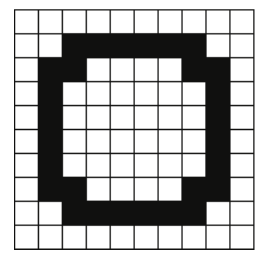
\includegraphics[scale=0.5]{images/img_zero.png}
	\end{center}

\end{Soln}
\begin{Soln}{8}
	~\\
	\begin{multicols}{2}
		\begin{enumerate}[label=\alph*)]
			\item  0 0 0 0 0 0\\
				   0 1 1 1 1 0\\
				   0 0 0 1 0 0\\
				   0 0 0 1 0 0\\
				   0 1 1 1 0 0\\
				   0 0 0 0 0 0\\

	        \item  0 0 0 0 1 0\\
	               0 0 0 0 1 1\\
	               0 1 1 1 1 0\\
	               0 1 0 1 0 0\\
	               0 1 0 1 0 0\\
	               0 0 0 0 0 0\\
	        \item  0 0 0 0 0 0 0 0 0 0 0 0 0\\
	               0 0 0 1 0 0 0 0 0 1 0 0 0\\
	               0 0 0 0 1 0 0 0 1 0 0 0 0\\
	               0 0 0 1 1 1 1 1 1 1 0 0 0\\
	               0 0 1 1 0 1 1 1 0 1 1 0 0\\
	               0 1 1 1 1 1 1 1 1 1 1 1 0\\
	               0 1 0 1 1 1 1 1 1 1 0 1 0\\
	               0 1 0 1 0 0 0 0 0 1 0 1 0\\
	               0 0 0 0 1 1 0 1 1 0 0 0 0\\
	               0 0 0 0 0 0 0 0 0 0 0 0 0\\
		\end{enumerate}
		\end{multicols}
\end{Soln}
\begin{Soln}{9}
	~\\	   \begin{center}
		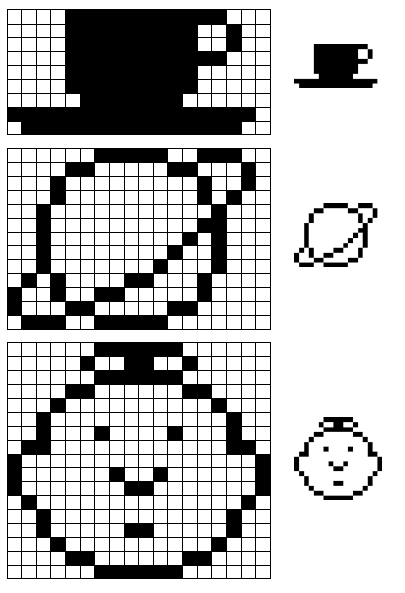
\includegraphics[scale=0.8]{images/corr_exo_code_imgBin_alt.png}
	\end{center}

\end{Soln}
